\documentclass[a4paper]{book}
\usepackage{lshort-zh-cn-style}
\newcommand{\code}{\ttfamily}
\usepackage{tikz}
\usetikzlibrary{chains,scopes,positioning,backgrounds,shapes,fit,shadows,calc,arrows.meta}
\usepackage{graphicx}
\usepackage{highlightlatex}
\usepackage{efbox}
\usepackage{verbatim}
\usepackage[skins]{tcolorbox} %必须标注skin,才能使用shadow命令显示阴影。
\tcbuselibrary{breakable} %breakable:支持跨页
\usepackage{xcolor}
\usepackage{amsmath}
\numberwithin{figure}{section}
\hypersetup{
	pdftitle={The Short Introduction to LaTeX2e (Chinese Simplified)},
	pdfkeywords={LaTeX, LaTeX2e},
	pdfcreator={XeLaTeX with `ctex' package},
}
%\title{\LaTeX 学习}
\author{huangzy1218}
\begin{document}
	\pdfbookmark{标题页}{title}
\thispagestyle{empty}

\vspace*{\stretch{1}}
\noindent\begin{minipage}{\textwidth}
\raggedleft
{\huge \bfseries ~\LaTeXe{}~Tutorial}
\noindent\rule[-1ex]{\textwidth}{5pt}\\[2.5ex]
\hfill\emph{\Large 记录我的\LaTeX{}学习过程}
\end{minipage}

\vspace{\stretch{1}}
\noindent\rlap{%
  \begin{minipage}{\textwidth}
  \linespread{2}\selectfont\raggedleft
  \makebox[2cm][l]{{\bfseries 笔\qquad 者:}}\makebox[4cm][l]{\bfseries 黄正阳}\\
  \makebox[2cm][l]{{\bfseries 邮\qquad 箱:}}\makebox[4cm][l]{\href{huangzy@nwafu.edu.cn}{huangzy@nwafu.edu.cn}}\\
  \makebox[2cm][l]{{\bfseries GitHub:}}\makebox[4cm][l]{\href{https://github.com/huangzy1218}{https://github.com/huangzy1218}}
  \end{minipage}%
}


	
	\frontmatter
	\tableofcontents

	\chapter{绘图功能}\label{chap:graphics}
\addtocontents{los}{\protect\addvspace{10pt}}
\section{\LaTeX{}绘图简介}
\LaTeX{} 提供了原始的picture 环境,能够绘制一些基本的图形如点、线、矩形、圆、Bézier
曲线等等,不过受制于\LaTeX{} 本身,它的绘图功能极为有限,效果也不够美观。

当前主流的\LaTeX{}绘图宏包/程序主要有:
\begin{itemize}
  \item PSTricks \par
以 PostSciprt 语法为基础的绘图宏包,具有优秀的绘图能力。它对老式的 \texttt{latex + dvips} 编译命令支持最好,
而现在的几种编译命令下使用起来都不够方便。

\item \hologo{TikZ} \& \pkg{pgf} \par
德国的 Till Tantau 教授在开发著名的 \LaTeX{} 幻灯片文档类 \cls{beamer} 时一并开发了绘图宏包 \pkg{pgf},
目的是令其能够在 \texttt{pdflatex} 或 \texttt{xelatex} 等不同的编译命令下都能使用。
\hologo{TikZ} 是在 \pkg{pgf} 基础上封装的一个宏包,采用了类似 \hologo{METAPOST} 的语法,提供了方便的绘图命令,绘图能力不输 PSTricks。

\item \hologo{METAPOST} \& Asymptote \par
\hologo{METAPOST} 脱胎于高德纳为 \TeX{} 配套开发的字体生成程序 \hologo{METAFONT},
具有优秀的绘图能力,并能够调用 \TeX{} 引擎向图片中插入文字和公式。
Asymptote 在 \hologo{METAPOST} 的基础上更进一步,具有一定的类似 C 语言的编程能力,支持三维图形的绘制。\par
它们作为独立的程序,通常的用法是将代码写在单独的文件里,编译生成图片供 \LaTeX{} 引用,也可以借助特殊的宏包在 \LaTeX{} 代码里直接使用。
\end{itemize}
\section{\hologo{TikZ} 绘图语言}
\subsection{绘图方式}
在导言区引入tikz宏包,就可使用命令或环境进行绘图操作。
\begin{itemize}
	\item 命令模式
	\begin{command}
		\cmd{tikz}\oarg*{...} \Arg{tikz code}\texttt{;} \\[1ex]
	\end{command}
	\item 命令分组模式
	\begin{command}
		\cmd{tikz}\oarg*{...} \marg*{\Arg{tikz code 1}\texttt{;} \Arg{tikz code 2}\texttt{;} ...} \\[1ex]
	\end{command}
	\item 环境模式
	\begin{command}
		\cmd{begin}\marg*{tikzpicture}\oarg*{...}\\
		\Arg{tikz code 1}\texttt{;}\\
		\Arg{tikz code 2}\texttt{;}\\
		\texttt{...}\\
		\cmd{end}\marg*{tikzpicture}\\
	\end{command}
	\item 起止命令模式
	\begin{command}
		\cmd{tikzpicture}\\
		\Arg{tikz code 1}\texttt{;}\\
		\Arg{tikz code 2}\texttt{;}\\
		\texttt{...}\\
		\cmd{endtikzpicture}
	\end{command}
\end{itemize}
 \begin{example}
  \tikz \draw(0,0) -- (1,1);
  \tikz{
   \draw(0,0) -- (1,1); 
    \draw(0,1) -- (1, 0)}
  \begin{tikzpicture} 
	\draw (-1,0) -- (1,0); 
	\draw (0,-1) -- (0,1); 
  \end{tikzpicture}
  \tikzpicture
   \draw (0,0) --(1,1);
   \draw (0,1) -- (1,0);
  \endtikzpicture
 \end{example}
\subsection{\hologo{TikZ}坐标}
\hologo{TikZ} 用直角坐标系或者极坐标系描述点的位置。

\begin{itemize}
	\item 直角坐标下,点的位置写作 \texttt{(\Arg{$x$},\Arg{$y$})},坐标 \Arg{$x$} 和 \Arg{$y$} 可以用 \LaTeX{} 支持的任意单位表示,
	缺省为 \texttt{cm};
	\item 极坐标下,点的位置写作 \texttt{(\Arg{$\theta$}:\Arg{r})}。$\theta$ 为极角,单位是度。
\end{itemize}
 使用绝对坐标
 \begin{example}
  \begin{tikzpicture}
   \draw (0,1) -- (1,0);
  \end{tikzpicture}
 \end{example}
 使用坐标单位,默认为cm,此时为绝对坐标
	\begin{example}
		\begin{tikzpicture}
			\draw (0pt,30pt) -- (30pt,0pt);
		\end{tikzpicture}
	\end{example}
 使用相对坐标,即相对第一个坐标的偏移
	\begin{example}
		\begin{tikzpicture}
			\draw (0,1) -- +(1,-1);
		\end{tikzpicture}
	\end{example}
	记录相对坐标,使用$++$ 
	\begin{example}
		\begin{tikzpicture}
			\draw (0,1) -- ++(1,-1) -- +(1,1);
		\end{tikzpicture}
	\end{example}
    使用极坐标,单位为°
	\begin{example}
		\begin{tikzpicture}
			\draw (90:1) -- (0:1) -- (2:1);
		\end{tikzpicture}
	\end{example}
	使用\cmd{usetikzlibrary}\marg*{calc}载入calc 扩展,可对坐标进行计算:
	\begin{example}
		\begin{tikzpicture}
			\draw (0,1) --($(0,1)-2*(-1,1)$);
		\end{tikzpicture}
	\end{example}
\subsection{\hologo{TikZ}路径}
\subsubsection{线段和折线}
若需要连续绘制,可连续使用--:
	\begin{example}
		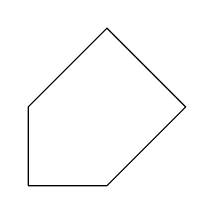
\begin{tikzpicture}
			\draw (0,0) -- (0,1) -- (1,2)
			-- (2,1) -- (1,0) -- (0,0);
		\end{tikzpicture}
	\end{example}
我们还可以为某个点命名:\cmd{coordinate} \texttt{(A) at (\Arg{coordinate})}
然后就可以使用 \texttt{(A)} 作为点的位置了。

\begin{example}
	\begin{tikzpicture}
		\draw (0,0) -- (30:1);
		\draw (1,0) -- (2,1);
		\coordinate (S) at (0,1);
		\draw (S) -- (1,1);
	\end{tikzpicture}
\end{example}
坐标的表示形式还包括“垂足”形式:
	\begin{example}
		\begin{tikzpicture}
			\draw (0,0) |- (1,1);
			\draw (1,0) -| (2,1);
		\end{tikzpicture}
	\end{example}
设置环境的默认参数\oarg*{line width}可改变线宽:
	\begin{example}
		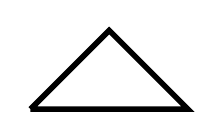
\begin{tikzpicture}[line width=
			2pt]
			\draw (0,0) -- (1,1) 
			-- (2,0) -- (0,0);
		\end{tikzpicture}
	\end{example}
由上例发现图形存在缺口,可通过\texttt{cycle}命令令路径回到起点,生成闭合的路径。
	\begin{example}
		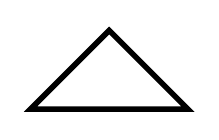
\begin{tikzpicture}[line width=
			2pt]
			\draw (0,0) -- (1,1) 
			-- (2,0) -- cycle;
		\end{tikzpicture}
	\end{example}
其它常用的路径还包括:
\begin{itemize}
	\item 矩形
\end{itemize}
	\begin{example}
		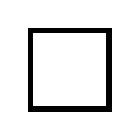
\begin{tikzpicture}[line width=
			2pt]
			\draw (0,0) rectangle (1,1);
		\end{tikzpicture}
	\end{example}
\begin{itemize}
	\item 网格、函数图像,网格可用 \texttt{step} 参数控制网格大小,函数图像用 \texttt{domain} 参数控制定义域:
\end{itemize}
	\begin{example}
		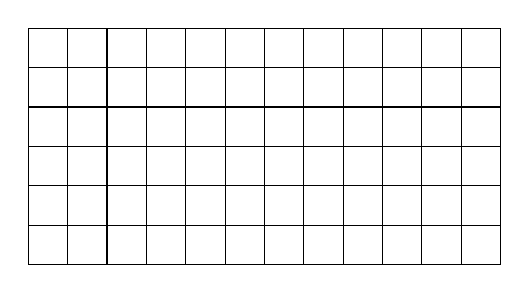
\begin{tikzpicture}
			% step指明网格间隔
			\draw[step=0.5](0,0) grid (6,3);
		\end{tikzpicture}
	\end{example}
\subsubsection{曲线}
绘制圆时,需要指定圆心和半径参数;绘制椭圆时,则需要指定圆心,并通过\texttt{ellipse}指定长轴和短轴:
	\begin{example}
		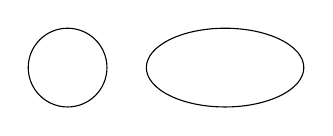
\begin{tikzpicture}
			\draw (0,0) circle (0.5);
			\draw (2,0) ellipse (1 and 0.5);
		\end{tikzpicture}
	\end{example}

使用\texttt{arc}绘制圆弧和椭圆弧:
	\begin{example}
		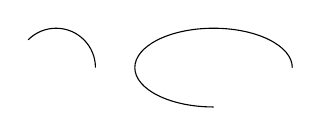
\begin{tikzpicture}
			\draw (0.5,0) arc (0:135: 0.5);
			\draw (3,0) arc (0:270:1 and 0.5);
		\end{tikzpicture}
	\end{example}

使用\texttt{parabola}绘制抛物线,默认起始点为抛物线顶点, 设置可选参数\texttt{bend at end}选项以终结点为顶点。
	\begin{example}
		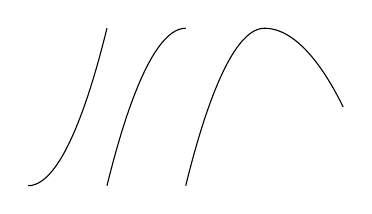
\begin{tikzpicture}
			\draw (0,0) parabola (1,2);
			\draw (1,0) parabola[bend at end] 
			(2,2);
			% 指定中间顶点坐标
			\draw (2,0) parabola bend
			(3,2) (4,1);
		\end{tikzpicture}
	\end{example}
使用\texttt{sin}和\texttt{cos}绘制三角函数曲线:
	\begin{example}
		\begin{tikzpicture}
			\draw (0,0) sin (1,1) cos (2,1); 
		\end{tikzpicture}
	\end{example}
\subsection{\hologo{TikZ}绘图绘图命令和参数}
除了 \cmd{draw} 命令之外,\hologo{TikZ} 还提供了 \cmd{fill} 命令用来填充图形,\cmd{filldraw} 命令则同时填充和描边。
以下示例常用的一些绘图命令和参数:
\begin{itemize}
	\item 
	\begin{command}
	\cmd{draw}\oarg*{color}
	\end{command}
\end{itemize}
	\begin{example}
		\begin{tikzpicture}
			\draw (0,0) rectangle (1,1);
			\draw[blue] (3,0) rectangle (4,1);
		\end{tikzpicture}
	\end{example}
\begin{itemize}
	\item
	\begin{command}
		\cmd{fill}\oarg*{color}
	\end{command} 
\end{itemize}
\begin{example}
	
\begin{tikzpicture}
		\fill (0,0.5) circle (0.5);
		\fill[yellow] (3,0.5) circle[radius=0.5];
	\end{tikzpicture}
\end{example}
\begin{itemize}
	\item 
	\begin{command}
		\cmd{filldraw}\oarg*{fill=color,draw=color}
	\end{command}
\end{itemize}
	\begin{example}
		
\begin{tikzpicture}
			\filldraw[fill=orange,draw=red]
			(0,0) rectangle (4.5,1);
		\end{tikzpicture}
	\end{example}
\begin{itemize}
\item 
\begin{command}
\cmd{shade}\oarg*{inner color=color,outer color=color}\\
\cmd{shade}\oarg*{left color=color,right color=color}
\end{command}
\end{itemize}
	\begin{example}
		
\begin{tikzpicture}
			\shade[inner color=yellow,
			outer color=orange]
			(1,1) circle (1);
			\shade[left color=gray,
			right color=black]
			(3,0) rectangle (4.5,2);
		\end{tikzpicture}
	\end{example}
\begin{itemize}
	\item \texttt{thick=\Arg{length}/thin/semithick/...} 指定线条的粗细:
\end{itemize}
\begin{example}
	
\begin{tikzpicture}
		\draw[ultra thin] (0,0)--(3,0);
		\draw[very thin] (0,1)--(3,1);
		\draw[thin] (0,2)--(3,2);
		\draw[semithick] (0,3)--(3,3);
		\draw[thick] (0,4)--(3,4);
		\draw[very thick] (0,5)--(3,5);
		\draw[ultra thick] (0,6)-- (3,6);
	\end{tikzpicture}
\end{example}
\begin{itemize}
	\item \texttt{solid/dashed/dotted/dash dot/dash dot dot} 指定线条类型(实线、虚线、点划线等)。
	与 \texttt{dashed} 对应地有 \texttt{densely dashed} 和 \texttt{loosely dashed},后三种类型同理。
\end{itemize}
\begin{example}
	\begin{tikzpicture}
		\draw[dashed] (0,0) -- (0,2);
		\draw[dotted] (0.5,0) -- (0.5,2);
		\draw[dash dot] (1,0) -- (1,2);
		\draw[dash dot dot] (1.5,0) -- (1.5,2);
		\draw[densely dotted]
		(2,0) -- (3,2) -- (4,0) -- cycle;
	\end{tikzpicture}
\end{example}
\begin{itemize}
	\item \texttt{\Arg{arrow}-\Arg{arrow}} 指定线条首尾的箭头形式。
	复杂的箭头形式需要在导言区使用 \cmd{use\-tikz\-library} \marg*{arrows.meta}。
\end{itemize}
\begin{example}
	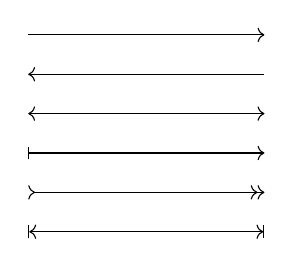
\begin{tikzpicture}
		\draw[->] (0,2.5) -- (3,2.5);
		\draw[<-] (0,2) -- (3,2);
		\draw[<->] (0,1.5) -- (3,1.5);
		\draw[|->] (0,1) -- (3,1);
		\draw[>->>] (0,0.5) -- (3,0.5);
		\draw[|<->|] (0,0) -- (3,0);
	\end{tikzpicture}
\end{example}
\begin{itemize}
	\item \texttt{rounded corners\oarg*{=\Arg{radius}}/sharp corners} 将路径转向处绘制成圆角/直角。可选参数 \Arg{radius} 控制圆角的半径。
	可以对某一段路径直接使用。
\end{itemize}
\begin{example}
	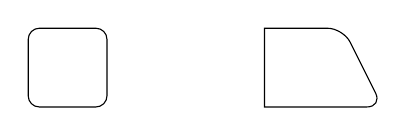
\begin{tikzpicture}
	\draw[rounded corners] 
	(0,0) rectangle (1,1);
	\draw (3,0)--(3,1) 
	[rounded corners=.2cm] 
	--(4,1)--(4.5,0)
	[sharp corners]--cycle; 
	\end{tikzpicture}
\end{example}
\begin{itemize}
	\item \texttt{scale/xshift/yshift/xslant/yslant/rotate} 设定图形的缩放、位移和旋转。
\end{itemize}
\begin{example}
	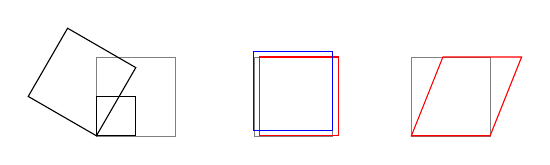
\begin{tikzpicture}
	\draw[help lines] (0,0) rectangle (1,1);
	\draw[scale=0.5] rectangle (1,1);
	\draw[rotate=60] rectangle (1,1);
	\draw[help lines] (2,0) rectangle (3,1);
	\draw[xshift=2pt,color=red] 
	(2,0) rectangle (3,1);
	\draw[yshift=2pt,color=blue] 
	(2,0) rectangle (3,1);
	\draw[help lines](4,0) rectangle (5,1);
	\draw[xslant=0.4,color=red]
	(4,0) rectangle (5,1);
	\end{tikzpicture}
\end{example}

为了重复利用绘图参数,减少代码冗余,\hologo{TikZ} 引入了“样式”的概念,可以定义一个样式包含绘图参数,
然后将样式作为一个参数用于绘图:
\begin{example}
	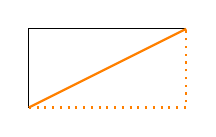
\begin{tikzpicture}
		[myarrow/.style={orange,thick}]
		\draw (0,0)--(0,1)--(2,1);
		\draw[myarrow] (0,0)--(2,1);
		\draw[myarrow,dotted]
		(0,0)--(2,0)--(2,1);
	\end{tikzpicture}
\end{example}

\envindex[tikz]{scope}
\hologo{TikZ} 还提供了 \env{scope} 环境,令绘图参数或样式在局部生效:
\begin{example}
	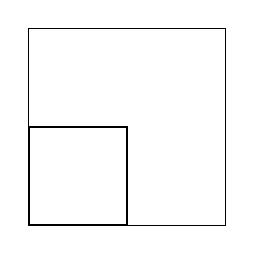
\begin{tikzpicture}
		\draw (0,0) rectangle (2.5, 2.5);
		\begin{scope}[thick,scale=0.5]
			\draw (0,0) rectangle (2.5, 2.5);
		\end{scope}
	\end{tikzpicture}
\end{example}

\subsection{文字节点}
使用\cmd{node}命令,基本格式如下:
\begin{command}
	\cmd{node}\oarg{options} \texttt{(\Arg{name})} \texttt{at (\Arg{coordinate})} \marg{text}\texttt{;}
\end{command}
\texttt{(\Arg{name})} 为结点命名,类似 \cmd{coordinate};\texttt{at (\Arg{coordinate})} 指定结点的位置。
这两者和前面的 \Arg{options} 都可以省略,只有 \Arg{text} 是必填的。
 
\Arg{options}可选择\texttt{left、right、above、below},若不指明位置,则结点文本中心与其结点坐标重合。
\begin{example}
 \begin{tikzpicture}
 	\draw[->] (0,0)--(5,0);
 	\draw[->] (0,-1.5)--(0,1.5);
 	\node[below,left] at (0,0) {$O$};
 	\node[right] at (5,0) {$x$};
 	\node[above] at (0,1.5) {$y$};
 	\draw (0,0) sin (1,1) cos (2,0)
 	 sin (3,-1) cos (4,0) ;
 \end{tikzpicture}
\end{example}
\begin{example}
	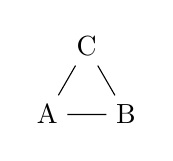
\begin{tikzpicture}
		\node (A) at (0,0) {A};
		\node (B) at (1,0) {B};
		\node (C) at (60:1) {C};
		\draw (A)--(B)--(C)--(A);
	\end{tikzpicture}
\end{example}
\cmd{node} 可指定特定的参数:
\begin{itemize}
	\item \oarg*{{anchor=\Arg{position}}} 令结点的某个角落 \Arg{position} 与 \Arg{coordinate} 对应。
	\item \oarg*{\texttt{centered / above / below / left / right / above left / ... \oarg*{=\Arg{length}}}} \\
	与 \texttt{anchor} 等效的选项。可选的 \Arg{length} 为结点相对于 \Arg{coordinate} 的距离。
\end{itemize}
\begin{example}
	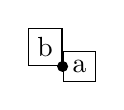
\begin{tikzpicture}
		\coordinate (A) at (1,1);
		\fill (A) circle[radius=2pt];
		\node[draw,anchor=west] at (A) {a};
		\node[draw,above left] at (A) {b};
	\end{tikzpicture}
\end{example}
\begin{itemize}
	\item \oarg*{\texttt{shape=\Arg{shape}}}
	结点的形状,默认可用 \texttt{rectangle} 和 \texttt{circle},可省略 \texttt{shape=} 直接写。在导言区使用命令
	\cmd{use\-tikz\-library}\marg*{shapes.geometric} 可用更多的形状。
	\item \oarg*{\texttt{text=\Arg{color}}}
	结点文字的颜色。
	\item \oarg*{\texttt{node font=\marg*{\Arg{font command}}}}
	结点文字的字体,形如 \cmd{bfseries} 或 \cmd{itshape} 等。
\end{itemize}
\begin{example}
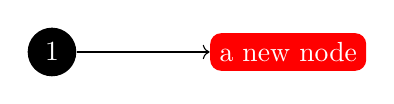
\begin{tikzpicture}
\node[circle,fill=black,text=white] 
(A) at (0,0) {1};
\node[rectangle,rounded corners,
color=white,fill=red] (B)
at (3,0) {a new node};
\draw[->] (A)--(B);
\end{tikzpicture}
\end{example}

\begin{itemize}
	\item \oarg*{\texttt{inner sep=\Arg{length} / outer sep=\Arg{length}}}
	结点边界向外和向内的额外距离。
	\item \oarg*{\texttt{minimum size=\Arg{length} / minimum height=\Arg{length} / minimum width=\Arg{length}}} \\
	结点的最小大小或最小高度/宽度。
\end{itemize}
\begin{example}
	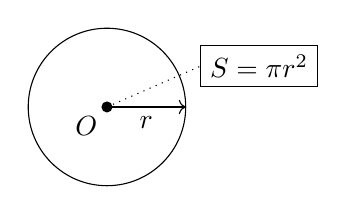
\begin{tikzpicture}
		\draw (0,0) circle[radius=1];
		\fill (0,0) circle[radius=2pt];
		\node[draw] (P) at (15:2) 
		{$S = \pi r^2$};
		\draw[->] (0,0)--(1,0);
		\node[below] at (0.5, 0) {$r$};
		\node[below left] at (0,0) {$O$};
		\draw[dotted] (0,0) -- (P.west);
	\end{tikzpicture}
\end{example}
节点之间使用相对位置,需引入\texttt{kzlibrary{positioning}}库。
\begin{example}
	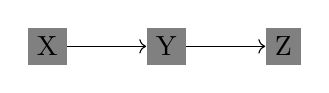
\begin{tikzpicture}
		\node[fill=gray] (a) {X};
		\node[fill=gray,right=1 of a] (b) {Y};
		\node[fill=gray,right=1 of b] (c) {Z};
		\draw[->] (a)--(b);
		\draw[->] (b)--(c);
	\end{tikzpicture}
\end{example}


\begin{sourcecode}[htp]
	\begin{Verbatim}
\begin{tikzpicture}[node distance=1cm]
% 定义流程图具体形状
 \tikzstyle{startstop} = [rectangle, rounded corners,thick, 
 minimum width=1cm, minimum height=0.5cm,text centered, 
 draw=black, fill=white,text width=1cm] % 开始
 \tikzstyle{process} = [rectangle,thick, minimum width=3cm, 
 minimum height=0.5cm, text centered, 
 draw=black, fill=white,text width=3cm]	% 步骤
 \tikzstyle{decision} = [diamond,aspect = 4, thick, minimum width=3cm, 
 minimum height=0.5cm, text centered, draw=black, fill=white]% 判断框
 \tikzstyle{arrow} = [thick,->,>=stealth]	% 箭头
 \node (start) [startstop] {开始};
 \node (pro1) [process, below of=start] {创建初始群};
 \node (pro2) [process, below of=pro1] {适应度计算};
 \node (dec1) [decision, below of=pro2,yshift=-0.38cm] {满足终止准则?};
 \node (pro3) [process, below of=dec1,yshift=-0.38cm] {选择操作};
 \node (pro4) [process, below of=pro3] {交叉操作};
 \node (pro5) [process, below of=pro4] {变异操作};
 \node (pro6) [process, right of=pro3,xshift=3cm] {变异操作};
 \node (stop) [startstop, below of=pro6] {结束};

 % 连接具体形状
 \draw [arrow](start) -- (pro1);
 \draw [arrow](pro1) -- (pro2);
 \draw [arrow](pro2) -- (dec1);
 \draw [arrow](dec1) -- (pro3);
 \draw [arrow](pro3) -- (pro4);
 \draw [arrow](pro4) -- (pro5);
 \draw [arrow](pro5) -| (-3,-2) |- (pro2);
 \draw [arrow](dec1) -| (pro6);
 \draw [arrow](pro6) -- (stop);
\end{tikzpicture}
	\end{Verbatim}
	\begin{center}
	\begin{tikzpicture}[node distance=1cm]
		% 定义流程图具体形状
		\tikzstyle{startstop} = [rectangle, rounded corners,thick, minimum width=1cm, minimum height=0.5cm,text centered, draw=black, fill=white,text width=1cm]	% 定义开始结束
		\tikzstyle{process} = [rectangle,thick, minimum width=3cm, minimum height=0.5cm, text centered, draw=black, fill=white,text width=3cm]	% 定义步骤
		\tikzstyle{decision} = [diamond,aspect = 4, thick, minimum width=3cm, minimum height=0.5cm, text centered, draw=black, fill=white]	% 定义判断框
		\tikzstyle{arrow} = [thick,->,>=stealth]	% 定义箭头
		\node (start) [startstop] {开始};
		\node (pro1) [process, below of=start] {创建初始群};
		\node (pro2) [process, below of=pro1] {适应度计算};
		\node (dec1) [decision, below of=pro2,yshift=-0.38cm] {满足终止准则?};
		\node (pro3) [process, below of=dec1,yshift=-0.38cm] {选择操作};
		\node (pro4) [process, below of=pro3] {交叉操作};
		\node (pro5) [process, below of=pro4] {变异操作};
		\node (pro6) [process, right of=pro3,xshift=3cm] {变异操作};
		\node (stop) [startstop, below of=pro6] {结束};
		
		% 连接具体形状
		\draw [arrow](start) -- (pro1);
		\draw [arrow](pro1) -- (pro2);
		\draw [arrow](pro2) -- (dec1);
		\draw [arrow](dec1) -- (pro3);
		\draw [arrow](pro3) -- (pro4);
		\draw [arrow](pro4) -- (pro5);
		\draw [arrow](pro5) -| (-3,-2) |- (pro2);
		\draw [arrow](dec1) -| (pro6);
		\draw [arrow](pro6) -- (stop);
	\end{tikzpicture}
	\end{center}
\end{sourcecode}
\begin{figure}[h]
\begin{center}
	\scalebox{0.6}{
\begin{tikzpicture}
	% 定义流程图具体形状
	\tikzstyle{startstop} = [rectangle,fill=blue!30, rounded corners,thick, minimum width=1cm, minimum height=0.5cm,text centered, draw=black,text width=1cm]	% 定义开始结束
	\tikzstyle{process} = [fill=yellow!30,rectangle,thick, minimum width=3cm, minimum height=0.5cm, text centered, draw=black,text width=3cm]	% 定义步骤
	\tikzstyle{decision} = [fill=green!30,diamond,aspect = 4, thick, minimum width=3cm, minimum height=0.5cm, text centered, draw=black]	% 定义判断框
	\tikzstyle{arrow} = [thick,->,>=stealth]	% 定义箭头
	\node (start) [startstop] {开始};
	\node (pro1) [process,below =0.6 of start]{初始化};%粒子的速%度和位置};
	\node (pro2) [process,below=0.6 of pro1]{计算每个粒子的适应度值};
	\node (pro3) [process,below=0.6 of pro2]{计算每个粒子的个体最优值};
	\node (pro4) [process,below=0.6 of pro3] {计算整群体的全局最优值};
	\node (pro5) [process,below=0.6 of pro4]{对粒子的速度、位置进行进化};
	\node (pro6) [process,below=0.6 of pro5]{进行边界条件处理};		
	\node (dec1) [decision,below=0.6 of pro6]{满足终止条件?};
	\node (pro7) [process,below=0.6 of dec1] {输出结果};
	\node (stop) [startstop,below=0.6 of pro7] {结束};
	
	% 连接具体形状
	\draw [arrow](start) -- (pro1);
	\draw [arrow](pro1) -- (pro2);
	\draw [arrow](pro2) -- (pro3);
	\draw [arrow](pro3) -- (pro4);
	\draw [arrow](pro4) -- (pro5);
	\draw [arrow](pro5) -- (pro6);
	\draw [arrow](pro6) -- (dec1);
	\draw[thick] (dec1.west) -| node[above]{\qquad \qquad 否}([xshift=-2cm]pro2.west) -| (pro2.west);
	\draw [arrow](dec1) -- (pro7);
	\draw [arrow] (pro7) to node[right] {是}  (stop);
\end{tikzpicture}}
	\caption{粒子群算法流程图}
\end{center}

\end{figure}
\subsection{绘制曲线}
\texttt{plot}操作绘制平面曲线,默认为描点连线:
\begin{example}
\begin{tikzpicture}
	\draw[->](0,0)--(4,0)node[right]{$x$};
	\draw[->](0,0)--(0,4)node[above]{$y$};
	% 画一般的平面曲线(描点连线)
	\draw plot coordinates
	{(0,0)(1,2)(2,1)(4,3)};
\end{tikzpicture}
\end{example}
若需要绘制光滑曲线,可使用\oarg*{smooth,tension}参数,其中\texttt{tension}指定紧绷度,取值范围从0到1,默认为0.55:
\begin{example}
 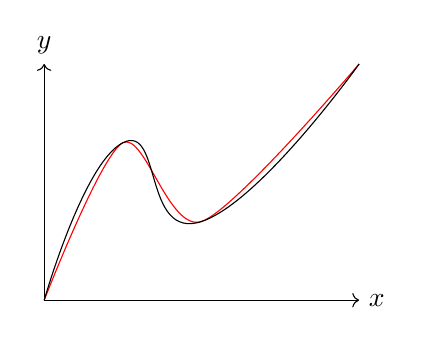
\begin{tikzpicture}
  \draw[->](0,0)--(4,0)node[right]{$x$};
  \draw[->](0,0)--(0,3)node[above]{$y$};
  \draw[color=red] plot[smooth] 
  coordinates {(0,0) (1,2) (2,1) (4,3)};
  \draw plot[smooth,tension=.9] 
  coordinates {(0,0) (1,2) (2,1) (4,3)};
 \end{tikzpicture}
\end{example}
\begin{example}
 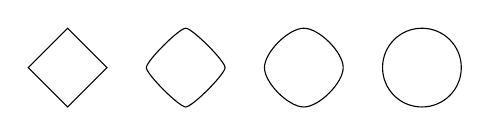
\begin{tikzpicture}[smooth cycle]
  \draw plot[tension=0] coordinates 
   {(0,0.5) (0.5,0) (1,0.5) (0.5,1)};
	% tension=0 将画出正方形,
	% 而tension=1 将画出圆形
  \draw[xshift=1.5cm] plot[tension=0.3] 
   coordinates
   {(0,.5) (.5,0) (1,.5) (.5,1)};
  \draw[xshift=3cm] plot[tension=0.7] 
   coordinates
   {(0,.5) (.5,0) (1,.5) (.5,1)};
  \draw[xshift=4.5cm] plot[tension=1] 
   coordinates
   {(0,.5) (.5,0) (1,.5) (.5,1)};
 \end{tikzpicture}
\end{example}
一般函数曲线通过\texttt{plot{\cmd{x},\cmd{y}}}绘制。
\begin{example}
 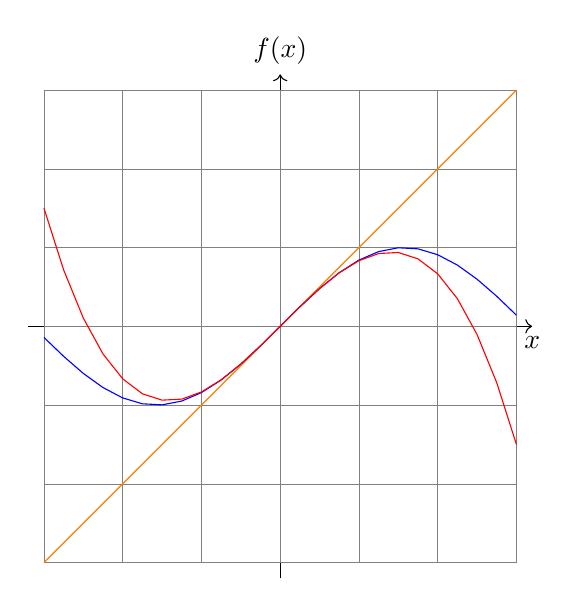
\begin{tikzpicture}[domain=-3:3]
  \draw[->] (-3.2,0) -- (3.2,0) 
   node[below] {$x$};
  \draw[->] (0,-3.2) -- (0,3.2) 
   node[above] {$f(x)$};
  \draw[very thin,color=gray] 
   (-3,-3) grid (3,3);
  \draw[color=orange]plot(\x,\x);
  \draw[color=blue]plot(\x,{sin(\x r)});
  \draw[color=red]plot(\x,
   {\x-(1/6)*(\x)^3});
 \end{tikzpicture}
\end{example}
Pgfplots是一个可视化工具,可以简化文档中的绘图。基本思想是提供输入数据/公式,而pgfplots完成其余工作。
\end{document}
